
	\section{ACM/ICPC World Finals 2008}
		\subsection{ACM/ICPC World Finals 2008 A Air Conditioning Machinery}
			\subsubsection{题目大意}
				如图 \ref{2008aaa},有一个 $N \times M \times K$  的空调。上有一个进风口一个出风口。试用不超过六个管道零件,拼接一个管道,至于空调\emph{内部},并连接两个风口,并输出最少需使用的管道数量。
					
				\begin{figure}[htb]
					\centering
					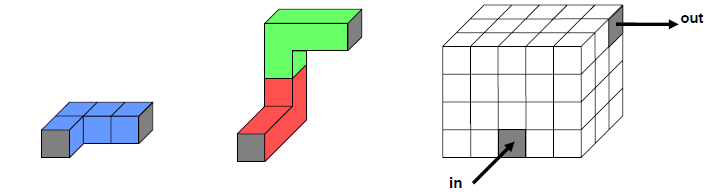
\includegraphics[width=0.7 \textwidth]{2008a.png}
					\caption{管道零件,管道,空调} \label{2008aaa}
				\end{figure}
			
			\subsubsection{算法讨论}
				暴力搜索,根据目前管子已经接到的位置,枚举下一个零件的方向(4 个),接长的一端还是短的一端(2 个)。注意管子不能超出空调外部,或与前面的管子重合。
					
				总搜索量不超过 $(4 \times 2) ^ 6$。
			
			
			\subsubsection{时空复杂度}
				
				时间复杂度 $\mathcal{O}\left(1\right)$。内含常数  $(4 \times 2) ^ 6 = \num{262144} $。
					
				空间复杂度 $\mathcal{O}\left(NMK\right)$。
		\newpage
		\subsection{ACM/ICPC World Finals 2008 B Always an Integer}
			\subsubsection{题目大意}
				给定若干形如
				\begin{align}
					P(x) = \frac{1}{b} \left( a_nx^n + a_{n - 1} x^{n - 1} + a_{n - 2} x^{n - 2}  + \cdots + a_{0} % x^{0} 
					  \right)
				\end{align}
				的 $n$ 次多项式,$a_i, b$ 均为整数。试问对于所有整数 $x \in \mathbb{Z}$ 是否都有 $P(x) \in \mathbb{Z}$。
				
				$n \le 100$。
			\subsubsection{算法讨论}
				\begin{theorem}
					$\forall x \in \mathbb{Z}, P(x) \in \mathbb{Z}$ 的充要条件是
					$\forall x \in \mathbb{Z} \cap [0, n], P(x) \in \mathbb{Z}$。
				\end{theorem}
				\begin{pf}
					后者的条件严于前者,故必要性显然,下证充分性。
					
%					将函数视为序列。
					定义差分 $\Delta [P](x) = P(x + 1) - P(x)$。再定义高阶差分 $\Delta^k [P](x) = \Delta^{k - 1} [P](x + 1) - \Delta^{k - 1} [P](x) $,特别地 $\Delta^0 [P](x) = P(x)$。
						
					容易验证,$\Delta^k [P](x), 0 \le k \le n$ 是一个 $(n - k)$ 次多项式,换言之,$\Delta^n [P](x)$ 是常函数。
					
					而如果确定了 $P(0), P(1), \ldots, P(n)$ 的值,就可以根据定义计算出 $\Delta^n [P](0)$ 指向的这个常数,从而推知整个 $\Delta^n [P](x)$,并倒推出所有 $\forall x \in \mathbb{Z}$ 的 $\Delta^{n - 1} [P](x) , \Delta^{n - 2} [P](x), \ldots$ ,直到原函数 $ \Delta^{0} [P](x)$。
					而整个过程我们只使用了对整数封闭的差分运算(加减运算),故只要一开始的 $P(0), P(1), \ldots, P(n)$  都是整数,那么 最终计算出的 $ \Delta^{0} [P](x)$ 所有整点就都是整数。% 故差分运算  $\Delta$ 对满足条件 
					\qed
				\end{pf}
				故我们只需对 $x \in \mathbb{Z} \cap [0, n]$ 进行检验。检验的方法是判断
				\begin{align}
					 \left( a_nx^n + a_{n - 1} x^{n - 1} + a_{n - 2} x^{n - 2}  + \cdots + a_{0} % x^{0} 
					  \right) \equiv 0 \pmod{b}
				\end{align}
				是否都成立,若是,答案则为是;反之答案为否。
			\subsubsection{时空复杂度}
				
				时间复杂度 $\mathcal{O}\left(n^2\right)$。
					
				空间复杂度 $\mathcal{O}\left(n\right)$。
		\newpage
		\subsection{ACM/ICPC World Finals 2008 C Conveyor Belt}
			\subsubsection{题目大意}
					如图 \ref{2008c},有若干齿轮,每个齿轮有规定的旋转方向。指定起点到终点,试用履带从起点连接到终点,使得
					\begin{enumerate}
						\item 符合齿轮旋转方向;
						\item 履带之间,以及履带和齿轮不交叉、重叠;
						\item 履带未与齿轮接触的部分,要求每一段的长度\emph{小于} $d$;且
						\item 履带总长最短。
					\end{enumerate}
					求这个总长度。
					
					齿轮数 $N \le 20$。
				\begin{figure}[htb]
					\centering
					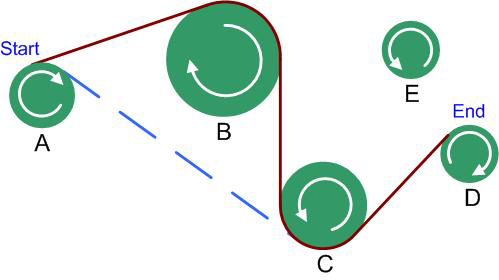
\includegraphics[width=0.6 \textwidth]{2008c.png}
					\caption{轮轴和履带} \label{2008c}
				\end{figure}
				
			\subsubsection{算法讨论}
				不妨先解决几何方面的问题。
				
				一个是两个轮轴间的连线,显然应为其公切线。具体是内公切线,还是外公切线,需根据两个轮轴的方向来确定。为讨论方便,可设顺时针的半径为负。这样设对应公切线的切点相对于圆心角度为 $\theta$,则应当满足方程
				
				\begin{align}
					((x_1 +r_1 \cos \theta)- (x_2 +r_2 \cos \theta), (y_1 +r_1 \sin \theta)-(y_2 +r_2 \sin \theta)) \cdot ( \cos \theta,  \sin \theta) = 0 \label{2008a}
				\end{align}
				因为切线应与圆心到切点的直线垂直。其中 $\cdot$ 是内积运算,$(a, b) \cdot (c, d) = ac + bd$。解  \eqref{2008a} 的方法是先化简为 
				\begin{align}
					(x_1 - x_2) \cos \theta + (y_1 - y_2) \sin \theta & = - (r_1 - r_2)
					\intertext{令 $d = \sqrt{(x_1 - x_2)^2 + (y_1 - y_2)^2}, (\cos \phi, \sin \phi) = ((x_1 - x_2) /d, (y_1 - y_2) / d)$,得}
					d \cos \left(\phi - \theta \right) & =  - (r_1 - r_2)
				\end{align}
				$\phi$ 和 $\theta$ 均可以用反三角求出。注意 $\theta$ 有两个解,具体取哪个根据方向确定。
				
				然后是线线和线圆的交叉的判定。前者用叉积即可判断。后者可以先将直线写成参数方程 $\mathbf{p} = \mathbf{a} + \mathbf{v} t$,代入圆方程 $ \left(\mathbf{p} - \mathbf{q}\right)^2 = r^2$,求解二次方程。根据解来判断。
					
				预处理好几何信息后,爆搜即可。注意需用交叉等减枝。
				
			\subsubsection{时空复杂度}
				时间复杂度 $\mathcal{O}\left(N^3\right)$ 几何预处理(此处没有履带交叉的检测) $+ $$ \mathcal{O}\left(N! N^2\right)$ 爆搜。题目限制繁多,致使实际有效状态并没有这么多。
					
				空间复杂度 $\mathcal{O}\left(N^2\right)$(某两个轮轴能否连边)。

		\newpage
		\subsection{ACM/ICPC World Finals 2008 E Huffman Codes}
			\subsubsection{题目大意}
				已知若干个字母的 Huffman 码,求有多少中频率分布能生成这样的  Huffman 码。约定频率为整百分数。频率小的都在左子树。
				
				字符数 $|\Sigma| = N \le 20$。
				
			\subsubsection{算法讨论}
				大致方向是爆搜。根据  Huffman 码,可以建立出  Huffman 树。
				
				约定右子树(1)优先访问,那么  Huffman 树的 BFS 序列的评论是单调下降的;反之亦然。具体的证明分两步。
				%可用调整法。
				第一步是要证明不同层的频率间大小关系的充要性,这个根据  Huffman 码构造时不断选择较小的频率合并不难证明,或者调整法,交换某两层的点后,会致使 Huffman 码不优(平均长度 $\sum{p_il_i}$ 没达到最小值);第二步是要说明同一层左边到右边的点的频率大小关系的充要性,这个是由于题目规定了频率小的都在左子树。此结论可以很大程度的加快搜索速度。
				
				随后爆搜就可以了。同一个父亲的两个节点的频率加起来要和父亲的相等,且须满足前面的结论。
				
			\subsubsection{时空复杂度}
				时间复杂度涉及到一个很困难的组合计数,并且还需考虑减枝,不易于表达成大 $\mathcal{O}$ 记法。不过考虑到 $N \le 20$,爆搜的速度应该还是很快的。
				
				空间复杂度 $\mathcal{O}\left(N\right)$。
			
		\newpage
		\subsection{ACM/ICPC World Finals 2008 F Glenbow Museum}
			\subsubsection{题目大意}	
				\begin{wrapfigure}{r}{0.25 \textwidth}
					\centering\vskip-2em
					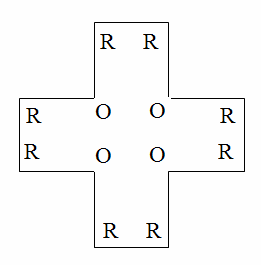
\includegraphics[width=0.23 \textwidth]{2008f.png}
					\caption{拐角表示法} \label{2008f}
				\end{wrapfigure}
					
				每个正交简单多边形,都可用如图所示的拐角表示法表示。(R)ight = 直角,(O)btuse = 钝角。逆时针将 RO 串起来得到的串就是 RO 串。
				
				定义一个 RO 串是需要计数的,当且仅当存在一个图形,其拐角表示法对应这个 RO 串,且内有一点可以“看”到所有边界。
				
				问所有的长度为 $N$ 的 RO 串中,有多少个是需要计数的。
				
			\subsubsection{算法讨论}

				\begin{theorem}
					问题等价于问所有的长度为 $N$ 的 RO 串中,有多少个的 R 比 O 多 4 个,且无连续两个 O。
				\end{theorem}
				\begin{pf}
					先说明 R 必须比 O 多 4 个。由于必须是简单多边形,故其旋转数为 $1$。分析可知,一个 R 的旋转数为 $\frac{1}{4}$ 而一个 O 的旋转数为 $-\frac{1}{4}$,故 R 必须比 O 多 4 个。
										\begin{figure}[htb]
					\centering
\definecolor{ffzzzz}{rgb}{1,0.6,0.6}
\definecolor{zzwwff}{rgb}{0.6,0.4,1}
\definecolor{zzttqq}{rgb}{0.6,0.2,0}
\definecolor{xdxdff}{rgb}{0.49,0.49,1}
\definecolor{qqqqff}{rgb}{0,0,1}
\definecolor{cqcqcq}{rgb}{0.75,0.75,0.75}



\centering
\begin{minipage}{.3\textwidth}
  \centering

\begin{tikzpicture}[line cap=round,line join=round,>=triangle 45,x=1.0cm,y=1.0cm,scale = 0.3]
\draw (4,20)-- (4,24);
\draw (4,24)-- (6,24);
\draw (6,24)-- (6,20);
\draw [->,color=ffzzzz] (4,22) -- (2,22);
\draw [->,color=ffzzzz] (6,22) -- (8,22);
\begin{scriptsize}
\if false
\fill [color=zzwwff] (4,20) circle (2.5pt);
\fill [color=zzwwff] (4,24) circle (2.5pt);
\fill [color=zzwwff] (6,24) circle (2.5pt);
\fill [color=zzwwff] (6,20) circle (2.5pt);
\fill [color=zzwwff] (2,22) circle (2.5pt);
\fill [color=zzwwff] (4,22) circle (2.5pt);
\fill [color=zzwwff] (6,22) circle (2.5pt);
\fill [color=zzwwff] (8,22) circle (2.5pt);
\fi

\end{scriptsize}

\end{tikzpicture}

  \captionof{figure}{}
  \label{fig:2008c1}
\end{minipage}%
\begin{minipage}{.7\textwidth}
  \centering
\definecolor{ffzzzz}{rgb}{1,0.6,0.6}
\definecolor{ttqqqq}{rgb}{0.2,0,0}
\definecolor{zzttqq}{rgb}{0.6,0.2,0}
\begin{tikzpicture}[line cap=round,line join=round,>=triangle 45,x=1.0cm,y=1.0cm, scale = 0.3]
\fill[color=zzttqq,fill=zzttqq,fill opacity=0.1] (1,6) -- (1,2) -- (2,2) -- (2,1) -- (5,1) -- (5,0) -- (9,0) -- (9,3) -- (10,3) -- (10,4) -- (11,4) -- (11,5) -- (10,5) -- (10,7) -- (3,7) -- (3,6) -- cycle;
\fill[color=zzttqq,fill=zzttqq,fill opacity=0.1] (14,6.8) -- (14,0.4) -- (14.2,0.4) -- (14.2,0.2) -- (14.4,0.2) -- (14.4,0) -- (23.6,0) -- (23.6,3) -- (23.8,3) -- (23.8,4) -- (24,4) -- (24,6.8) -- (23.8,6.8) -- (23.8,7) -- (14.2,7) -- (14.2,6.8) -- cycle;
\draw [color=zzttqq] (1,6)-- (1,2);
\draw [color=zzttqq] (1,2)-- (2,2);
\draw [color=zzttqq] (2,2)-- (2,1);
\draw [color=zzttqq] (2,1)-- (5,1);
\draw [color=zzttqq] (5,1)-- (5,0);
\draw [color=zzttqq] (5,0)-- (9,0);
\draw [color=zzttqq] (9,0)-- (9,3);
\draw [color=zzttqq] (9,3)-- (10,3);
\draw [color=zzttqq] (10,3)-- (10,4);
\draw [color=zzttqq] (10,4)-- (11,4);
\draw [color=zzttqq] (11,4)-- (11,5);
\draw [color=zzttqq] (11,5)-- (10,5);
\draw [color=zzttqq] (10,5)-- (10,7);
\draw [color=zzttqq] (10,7)-- (3,7);
\draw [color=zzttqq] (3,7)-- (3,6);
\draw [color=zzttqq] (3,6)-- (1,6);
\draw [color=zzttqq] (14,6.8)-- (14,0.4);
\draw [color=zzttqq] (14,0.4)-- (14.2,0.4);
\draw [color=zzttqq] (14.2,0.4)-- (14.2,0.2);
\draw [color=zzttqq] (14.2,0.2)-- (14.4,0.2);
\draw [color=zzttqq] (14.4,0.2)-- (14.4,0);
\draw [color=zzttqq] (14.4,0)-- (23.6,0);
\draw [color=zzttqq] (23.6,0)-- (23.6,3);
\draw [color=zzttqq] (23.6,3)-- (23.8,3);
\draw [color=zzttqq] (23.8,3)-- (23.8,4);
\draw [color=zzttqq] (23.8,4)-- (24,4);
\draw [color=zzttqq] (24,4)-- (24,6.8);
\draw [color=zzttqq] (24,6.8)-- (23.8,6.8);
\draw [color=zzttqq] (23.8,6.8)-- (23.8,7);
\draw [color=zzttqq] (23.8,7)-- (14.2,7);
\draw [color=zzttqq] (14.2,7)-- (14.2,6.8);
\draw [color=zzttqq] (14.2,6.8)-- (14,6.8);
\end{tikzpicture}
  \captionof{figure}{转化 的例子}
  \label{fig:2008c2}
\end{minipage}
\end{figure}

					再说明 不能有相邻的 O。原因也很简单,如果有,那么就能形成如图 \ref{fig:2008c1} 所示的图形,半平面交肯定为 $\varnothing$。
					
					最后说明只要 R 比 O 多 4 个,且无连续两个 O,就能找到这样的一个简单多边形。我们可以先随意画出一个拐角表示法为该序列的简单多边形。然后固定最靠上、下、左、右的边,通过将另外的边缩短为无穷小的方法,将其变化成一个趋近于长方形的图形。由于没有两个连续的 O ,故边界上也就没有无限小的内凹。此时只要这个图形无线趋近于长方形,那么其中点(重心)就无限趋近于满足要求。这个无限趋近于长方形的图形就是我们要找的。
				\end{pf}
				这样就变成了一个计数问题。如果 $N$ 为奇数,则答案为 $0$;否则答案
				\begin{align}
					Ans = \binom{N/2 + 1}{3} + 2 \binom{N/2 + 1}{4} \label{2008feq}
				\end{align}
				\eqref{2008feq} 的得出方法是通过枚举首尾的字母情况,再使用隔板法。
					
			\subsubsection{时空复杂度}
				时空复杂度 $\mathcal{O}\left(1\right)$。


		\newpage
\subsection{ACM/ICPC World Finals 2008 G Net Loss}
		\subsubsection{题意概述}
			给定多项式 $p(x)$ 和常数 $c \left(-1 < c < 1\right)$,求三个实数 $k_1,k_2,b$ 使得
			\begin{align}
				d = \int_{-1}^{c} \left(k_1\left(x-c\right)+b - p(x)\right)^2 \mathrm{d}x
					+ \int_{c}^{1} \left(k_2\left(x-c\right)+b - p(x)\right)^2 \mathrm{d}x 
			\end{align}
			最小化,并输出 $k_1,k_2,b$ 的值。
			
			$1 \le p(x) \text{的次数} \le 10$。多组询问。
			
		\subsubsection{简要分析}
			考虑 $d$ 关于 $k_1,k_2,b$ 的梯度
			\begin{align}
				\nabla d & = \left(\frac{\mathrm{\partial} d}{\mathrm{\partial} k_1},
						\frac{\mathrm{\partial} d}{\mathrm{\partial} k_2},
						\frac{\mathrm{\partial} d}{\mathrm{\partial} b}\right) 
			\end{align}
			其中
			\begin{align}
					\frac{\mathrm{\partial} d}{\mathrm{\partial} k_1} 
						& = \int_{-1}^{c} 2(k_1(x-c)+b-p(x)) \cdot (x-c) \; \mathrm{d}x\\
					\frac{\mathrm{\partial} d}{\mathrm{\partial} k_2} 
						& = \int_{c}^{1} 2(k_2(x-c)+b-p(x)) \cdot (x-c) \; \mathrm{d}x\\
					\frac{\mathrm{\partial} d}{\mathrm{\partial} b} 
						& = \int_{-1}^{c} 2(k_1(x-c)+b-p(x)) \; \mathrm{d}x +
							\int_{c}^{1} 2(k_2(x-c)+b-p(x)) \; \mathrm{d}x 
			\end{align}
			由三个方向的偏导随该维的单调性可知,$d$ 取得最小值当且仅当
			\begin{align}
				\nabla d = \mathbf{0}
			\end{align}
			即
			\begin{align}
				\left\{\setlength{\tabcolsep}{2.5pt}
					\begin{tabular}{cccccccc}
						$\displaystyle k_1 \int_{-1}^{c} (x-c)^2 \; \mathrm{d}x$ & $+$ & $0$ & $+$ & $\displaystyle b \int_{-1}^{c} (x-c) \; \mathrm{d}x $  &$ =$&$\displaystyle  \int_{-1}^{c} p(x)\cdot(x-c) \; \mathrm{d}x$ \\
						$0$ & $+$ & $\displaystyle k_2 \int_{c}^{1} (x-c)^2 \; \mathrm{d}x$ &$ +$&$ \displaystyle b \int_{c}^{1} (x-c) \; \mathrm{d}x $&$  =$ &$ \displaystyle \int_{c}^{1} p(x)\cdot(x-c) \; \mathrm{d}x$ \\
						$k_1 \displaystyle \int_{-1}^{c} (x-c) \; \mathrm{d}x$ & $+$ & $k_2\displaystyle \int_{c}^{1} (x-c) \; \mathrm{d}x$ &$ +$&$ b \displaystyle \int_{-1}^{1} \mathrm{d}x $&$  =$ &$ \displaystyle \int_{-1}^{1} p(x) \; \mathrm{d}x$ 
					\end{tabular}
				\right.
			\end{align}
			写成矩阵的形式
			\begin{align}
				A\mathbf{x} = \mathbf{b}
			\end{align}
			其中
			\begin{align}
				A & = \begin{bmatrix}
					\displaystyle \int_{-1}^{c} (x-c)^2 \; \mathrm{d}x & 0 & \displaystyle\int_{-1}^{c} (x-c) \; \mathrm{d}x \\
					0 & \displaystyle\int_{c}^{1} (x-c)^2 \; \mathrm{d}x &\displaystyle \int_{c}^{1} (x-c) \; \mathrm{d}x \\
					\displaystyle\int_{-1}^{c} (x-c) \; \mathrm{d}x & \displaystyle\int_{c}^{1} (x-c) \; \mathrm{d}x & 2
				\end{bmatrix} \\
				\mathbf{x} & = (k_1,k_2,b)^{\mathrm{T}} \\
				\mathbf{b} & = \left(\int_{-1}^{c} p(x)\cdot(x-c) \; \mathrm{d}x,
					\int_{c}^{1} p(x)\cdot(x-c) \; \mathrm{d}x,
					\int_{-1}^{1} p(x) \; \mathrm{d}x\right)^{\mathrm{T}}
			\end{align}
			定积分可以使用牛顿—莱布尼兹定理求得。剩下的只需使用高斯消元,人工解方程,或者通过伴随矩阵求逆矩阵等方法求出解向量 $\mathbf{x}$。
			
			计算可得,系数矩阵 $A$ 的行列式 $\left|A\right| = \textstyle \frac{1}{18} (1+c)^3 (1-c)^3 $,故 $\left|A\right|  > 0 $ 恒成立,方程组恒有且仅有一组解。
				
			\subsubsection{时空复杂度}
				时间复杂度 $\mathcal{O}\left(p(x) \text{的次数}\right)$。
				
				空间复杂度 $\mathcal{O}\left(p(x) \text{的次数}\right)$。
		
		\newpage
		\subsection{ACM/ICPC World Finals 2008 H Painter}
		\subsubsection{题意概述}
			如图  \ref{2008h} 有一堆三角形。判断三角形的边界是否有重叠(端点重合也算)。如果没有,再判断三角形迭代了最多几层。

				三角形数 $n \le 100000$。
				
				
				\begin{figure}[htb]
					\centering
					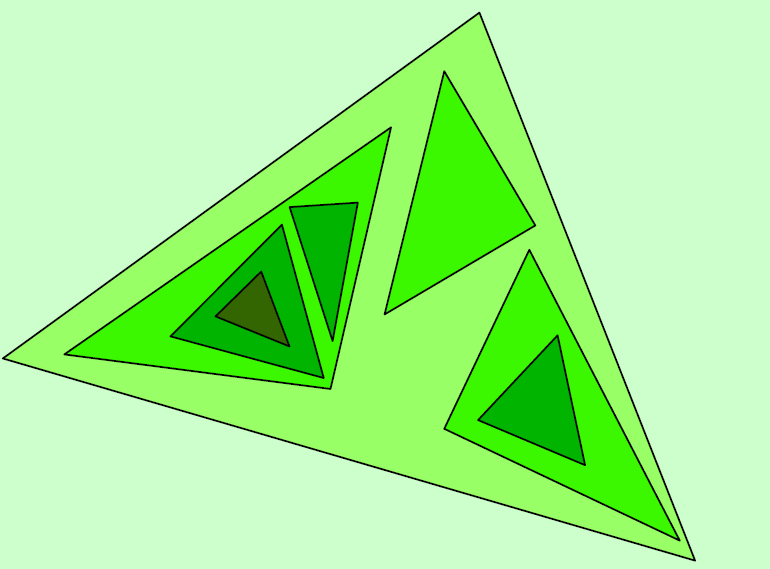
\includegraphics[width=0.4 \textwidth]{2008h.png}
					\caption{可能的三角形集} \label{2008h}
					\vskip-1em
				\end{figure}
				
		\subsubsection{简要分析}
				整个问题都可以用扫描线解决。
				
				设没有竖直的边(若有,则旋转某一角度),那么从左到右扫描,三角形就是一个从点,线性地变化为一个区间,再变成一个一个点,最后消失的动态区间。而同理直线就是动点。
				
				不妨用平衡树来维护整个扫描线,那么一个新三角形出现在扫面线上时,需要加两个动点。为了避免交叉,需要与其前一个和后一个动点所在的直线进行交叉检测。而对于其他点,我们可以保证目前(在前一个点或后一个点删除之前)不会交叉,因为如果交叉,其必然会与相邻点交叉,而不会跨过这两个点。
				
				同样地,删除时,需对待删除点的相邻两条直线先进行交叉检测,再删除。
				
				交叉检测使用叉积来判定,且 需小心处理端点。如果有任何一次的交叉检测不通过,那么就立即返回边界重叠,退出程序。
				
				如果没有重叠的边界,那么我们可以继续借助前面辅助线的信息,在插入三角形(两个动点)前维护其父子关系;或者我们只关心其深度,故维护好次深度即可。不妨将三角形的上边界看为 $+ 1$,下边界看为 $- 1$。那么要求得深度,只需对在当前三角形的上方的边界的权值求和就可以了。
				
				答案为所有三角形深度的最大值。
			\subsubsection{时空复杂度}
				时间复杂度 $\mathcal{O}\left(n \log n\right)$。
				
				空间复杂度 $\mathcal{O}\left(n\right)$。
		
		
		\newpage
		\subsection{ACM/ICPC World Finals 2008 J The Sky is the Limit}
			\subsubsection{题意概述}
				如图 \ref{2008j} 有很多\emph{等腰}三角形的山峰。计算其并集的轮廓中,不属于地面的长度。
			
				\begin{figure}[htb]
					\centering
					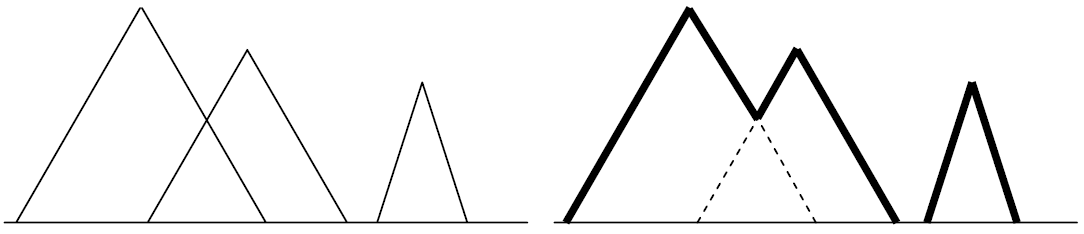
\includegraphics[width=0.9 \textwidth]{2008j.png}
					\caption{山坡与轮廓} \label{2008j}
					\vskip-1em
				\end{figure}
				
				山峰数 $N \le 100$。
			\subsubsection{简要分析}
				对于所有三角形,两两地求出其所有交点。加上端点,设总共有 $M$ 个 点,那么将这些点横坐标排序,就能将整个地面分成 $(M + 1)$ 部分。每一部分里,需要计算的“轮廓”都是直线,由区间端点上最高的处的位置连接而成。求出端点上的高度后,套用勾股定理求轮廓长度之和即可。
				
			\subsubsection{时空复杂度}
				$\mathcal{O}(M) =  \mathcal{O}\left(N^2\right)$,故时间复杂度
				$ \mathcal{O}\left(MN\right) = \mathcal{O}\left(N^3\right)$。
				
				空间复杂度 $\mathcal{O}\left(N^2\right)$。
				
				
		\newpage
			
			